\documentclass[12pt]{article}
\usepackage[margin=1in]{geometry}
\usepackage{amsmath, amssymb, amsthm, mathtools, bm}
\usepackage{booktabs}
\usepackage{enumitem}
\usepackage{microtype}
\usepackage{physics}
\usepackage{hyperref}
\hypersetup{colorlinks=true, linkcolor=blue, urlcolor=blue, citecolor=blue}

\usepackage{tikz}
\usetikzlibrary{arrows.meta,intersections,calc}
\usepackage{pgfplots}
\pgfplotsset{compat=1.15}


\newcommand{\R}{\mathbb{R}}
%\newcommand{\dd}{\,\mathrm{d}}
\newcommand{\pd}[2]{\frac{\partial #1}{\partial #2}}
\newcommand{\dtotal}[2]{\frac{\mathrm{d} #1}{\mathrm{d} #2}}
\newcommand{\argmax}{\operatorname*{arg\,max}}
\newcommand{\argmin}{\operatorname*{arg\,min}}

\theoremstyle{definition}
\newtheorem{definition}{Definition}
\newtheorem{example}{Example}
\newtheorem{remark}{Economist's Intuition}
\newtheorem{proposition}{Proposition}

\title{Optimization of Single-Variable Functions\\[10pts]
{\large ECON 320 - Introduction to Mathematical Economics}}
\author{Muhebullah Karimzada}
\date{Fall 2025}


% --- tcolorbox setup ---
\usepackage[most]{tcolorbox} % loads skins, theorems, raster, breakable, etc.
\tcbset{
    colback=blue!5!white,
    colframe=blue!50!black,
  sharp corners,
  boxrule=0.6pt,
  enhanced,
  breakable,
}











\begin{document}
\maketitle
\tableofcontents

\newpage

\section{Optimum Values and Extreme Values}

An economic agent chooses a scalar decision variable $x$ (output $Q$, advertising $A$, savings $s$, etc.) to maximize or minimize an objective function $y=f(x)$. The optimization target may be a \emph{relative} (local) extremum or an \emph{absolute} extremum over the domain.

\begin{definition}[Relative (Local) vs. Absolute Extremum]
Let $f:\mathcal{D}\subseteq\R\to\R$ and $x_0\in\mathcal{D}$. 
\begin{itemize}[leftmargin=1.5em]
\item $f(x_0)$ is a \emph{relative (local) maximum} if $\exists \varepsilon>0$ s.t. $f(x_0)\ge f(x)$ for all $x$ with $|x-x_0|<\varepsilon$.
\item $f(x_0)$ is a \emph{relative (local) minimum} if $\exists \varepsilon>0$ s.t. $f(x_0)\le f(x)$ for all $x$ with $|x-x_0|<\varepsilon$.
\item $f(x^\star)$ is an \emph{absolute maximum (minimum)} if $f(x^\star)\ge(\le)\, f(x)$ for all $x\in\mathcal{D}$.
\end{itemize}
\end{definition}

\begin{remark}
In many economic problems the domain is restricted (e.g., $Q\ge0$). Absolute optima may then occur at \emph{boundaries} (corner solutions). Always check feasible endpoints.
\end{remark}

\section{Relative Maximum and Minimum: First-Derivative Test}
\subsection*{Stationary points and the sign-change test}
If $f$ is differentiable, any interior relative extremum must occur at a \emph{stationary point} $x_0$ where
\[
f'(x_0)=0.
\]
This is \emph{necessary} but not sufficient: $f'(x_0)=0$ could also be an inflection point. The first-derivative \emph{sign-change} criterion turns necessity into a decision rule.

\begin{proposition}[First-Derivative Test]
Let $f$ be differentiable around $x_0$ with $f'(x_0)=0$.
\begin{itemize}[leftmargin=1.5em]
\item If $f'$ changes $+$ to $-$ when crossing $x_0$, then $x_0$ is a relative maximum.
\item If $f'$ changes $-$ to $+$ when crossing $x_0$, then $x_0$ is a relative minimum.
\item If $f'$ does not change sign across $x_0$, then $x_0$ is neither max nor min (typically an inflection).
\end{itemize}
\end{proposition}

\begin{example}[Cubic with two stationary points]
Let $f(x)=x^3-12x^2+36x+8$. Then $f'(x)=3x^2-24x+36=3(x-2)(x-6)$, so the stationary points are $x=2,6$.
A sign chart for $f'$ shows: on $( -\infty,2)$, $f'>0$; on $(2,6)$, $f'<0$; on $(6,\infty)$, $f'>0$. Hence
\[
x=2\text{ is a local maximum},\qquad x=6\text{ is a local minimum}.
\]
Evaluating: $f(2)=2^3-12(4)+72+8=8-48+72+8=40$, $f(6)=216-432+216+8=8$.
\end{example}

\begin{example}[Average cost minimization]
Average cost $AC(Q)=Q^2-5Q+8$. Then $AC'(Q)=2Q-5$, so the unique stationary point is $Q^\ast=2.5$. Check the sign change of $AC'$: negative for $Q<2.5$, positive for $Q>2.5$ $\Rightarrow$ $Q^\ast$ minimizes $AC$ and, for this quadratic, is also the absolute minimum.
\end{example}



\section{Second and Higher Derivatives}

The second derivative measures the rate of change of the slope:
\[
f''(x)=\dtotal{}{x}\!\big[f'(x)\big],\qquad
f^{(n)}(x)=\dtotal[n]{f(x)}{x}.
\]

\subsection*{Geometry and curvature}
\begin{itemize}[leftmargin=1.5em]
\item $f''(x)>0$ $\Rightarrow$ slope increasing: the graph is \emph{convex} (strictly convex if $f''>0$ on an interval).
\item $f''(x)<0$ $\Rightarrow$ slope decreasing: the graph is \emph{concave} (strictly concave if $f''<0$ on an interval).
\item At an \emph{inflection point} the curvature changes sign; $f'$ typically reaches a local extremum.
\end{itemize}

\begin{remark}[Risk attitudes]
In expected-utility models, a concave utility $U$ ($U''<0$) captures risk aversion; a convex utility ($U''>0$) captures risk loving. For a fair gamble with expected payoff $E[x]$, a risk-averse agent prefers the certain $E[x]$ to the lottery because diminishing marginal utility makes the utility of the gain smaller in absolute value than the utility loss of an equally likely loss.
\end{remark}

\begin{example}[Interpreting $f'$ and $f''$ numerically]
If $f'(x_0)=1.2$ and $f''(x_0)=-0.5$, then near $x_0$ the function is increasing ($f'>0$) but at a diminishing rate ($f''<0$): think increasing output with diminishing marginal returns.
\end{example}






%=============================
% Figure: Convexity (f'' > 0)
%=============================
\begin{figure}[ht]
\centering
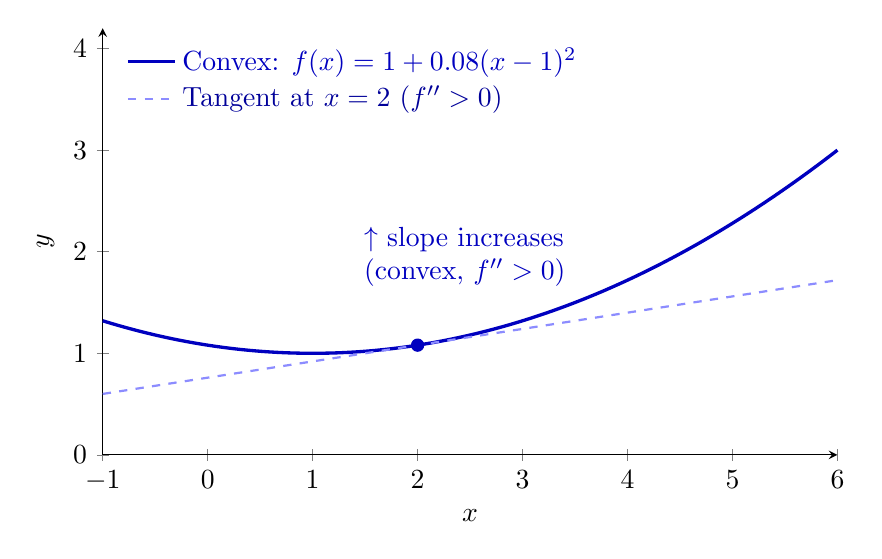
\begin{tikzpicture}
\begin{axis}[
  width=0.9\textwidth,
  height=7cm,
  xmin=-1, xmax=6,
  ymin=0,  ymax=4.2,
  axis lines=left,
  xlabel={$x$}, ylabel={$y$},
  legend style={at={(0.02,0.98)},anchor=north west, draw=none, fill=none},
  legend cell align=left,
  domain=-1:6, samples=200, clip=false
]

% Convex curve (blue) and its tangent (light blue)
\addplot[very thick, color=blue!75!black] {1 + 0.08*(x-1)^2};
\addlegendentry{\textcolor{blue!75!black}{Convex: $f(x)=1+0.08(x-1)^2$}}

% Tangent line at x=2: slope = 0.16, point (2,1.08)
\addplot[thick, dashed, color=blue!45!white] {0.76 + 0.16*x};
\addlegendentry{\textcolor{blue!60!black}{Tangent at $x=2$ ($f''>0$)}}

% Tangency point
\addplot[only marks, mark=*, mark size=2.2pt, color=blue!75!black] coordinates {(2,1.08)};

% Annotation
\node[align=left, text=blue!75!black] at (axis cs:2.45,1.95) {$\uparrow$ slope increases\\(convex, $f''>0$)};

\end{axis}
\end{tikzpicture}
\caption{Convexity ($f''>0$): the slope increases with $x$. The dashed line is the tangent at $x=2$.}
\end{figure}



%=============================
% Figure: Concavity (f'' < 0)
%=============================
\begin{figure}[ht]
\centering
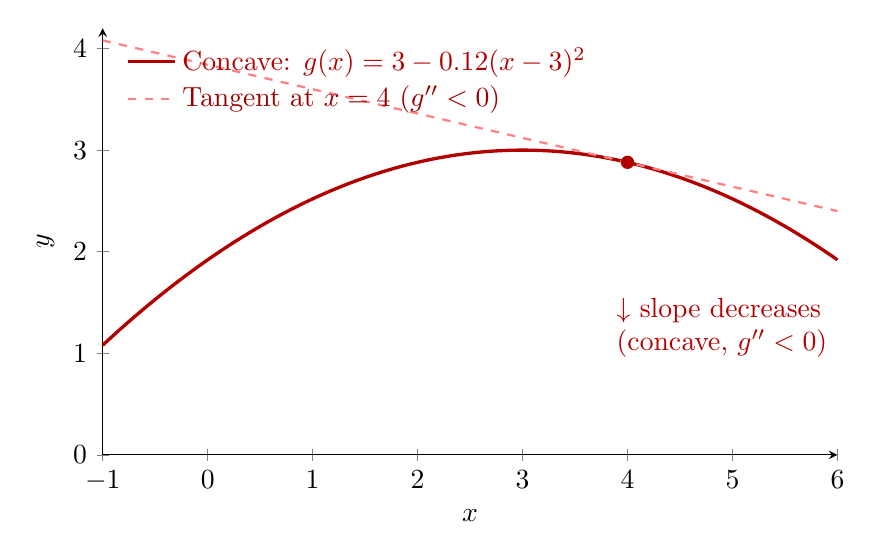
\begin{tikzpicture}
\begin{axis}[
  width=0.9\textwidth,
  height=7cm,
  xmin=-1, xmax=6,
  ymin=0,  ymax=4.2,
  axis lines=left,
  xlabel={$x$}, ylabel={$y$},
  legend style={at={(0.02,0.98)},anchor=north west, draw=none, fill=none},
  legend cell align=left,
  domain=-1:6, samples=200, clip=false
]

% Concave curve (red) and its tangent (light red)
\addplot[very thick, color=red!70!black] {3 - 0.12*(x-3)^2};
\addlegendentry{\textcolor{red!70!black}{Concave: $g(x)=3-0.12(x-3)^2$}}

% Tangent line at x=4: slope = -0.24, point (4,2.88)
\addplot[thick, dashed, color=red!50!white] {3.84 - 0.24*x};
\addlegendentry{\textcolor{red!60!black}{Tangent at $x=4$ ($g''<0$)}}

% Tangency point
\addplot[only marks, mark=*, mark size=2.2pt, color=red!70!black] coordinates {(4,2.88)};

% Annotation
\node[align=left, text=red!70!black]  at (axis cs:4.9,1.25)  {$\downarrow$ slope decreases\\(concave, $g''<0$)};

\end{axis}
\end{tikzpicture}
\caption{Concavity ($g''<0$): the slope decreases with $x$. The dashed line is the tangent at $x=4$.}
\end{figure}

\begin{tcolorbox}[sidebyside, righthand width=0.42\textwidth, title=\textbf{Convexity ($f''>0$)}]
\begin{minipage}{0.56\textwidth}
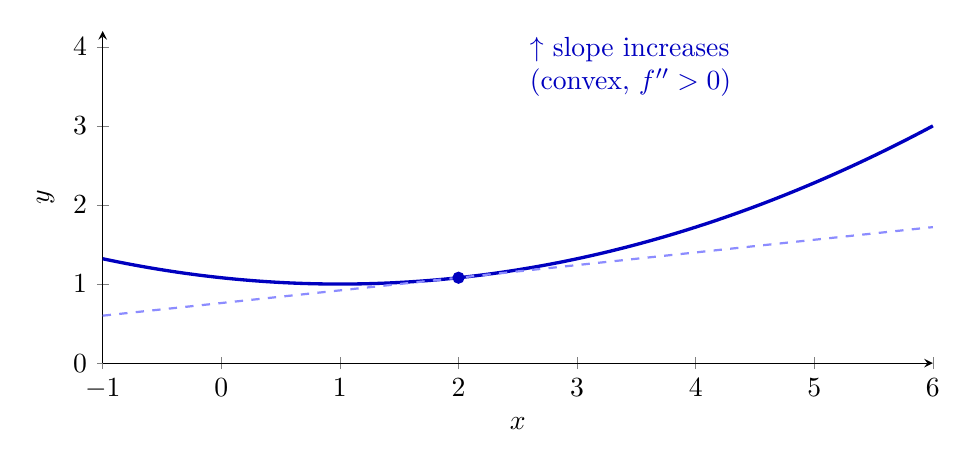
\begin{tikzpicture}
\begin{axis}[
  width=\linewidth, height=5.8cm,
  xmin=-1, xmax=6, ymin=0, ymax=4.2,
  axis lines=left, xlabel={$x$}, ylabel={$y$},
  domain=-1:6, samples=200, clip=false
]
\addplot[very thick, color=blue!75!black] {1 + 0.08*(x-1)^2};
\addplot[thick, dashed, color=blue!45!white] {0.76 + 0.16*x};
\addplot[only marks, mark=*, mark size=2pt, color=blue!75!black] coordinates {(2,1.08)};
\node[align=left, text=blue!75!black] at (axis cs:3.45,3.75) {$\uparrow$ slope increases\\(convex, $f''>0$)};
\end{axis}
\end{tikzpicture}
\end{minipage}
\tcblower
If $f'(x_0)=0$ and $f''(x_0)>0$, $x_0$ is a \emph{local minimum} (Chs.\ 9.3–9.4).  
When $f''(x_0)=0$ is inconclusive, use the sign change of $f'$ (Ch.\ 9.2) or the $n$th-derivative test (Ch.\ 9.6).
\end{tcolorbox}

\begin{tcolorbox}[sidebyside, righthand width=0.42\textwidth, title=\textbf{Concavity ($f''<0$)}]
\begin{minipage}{0.56\textwidth}
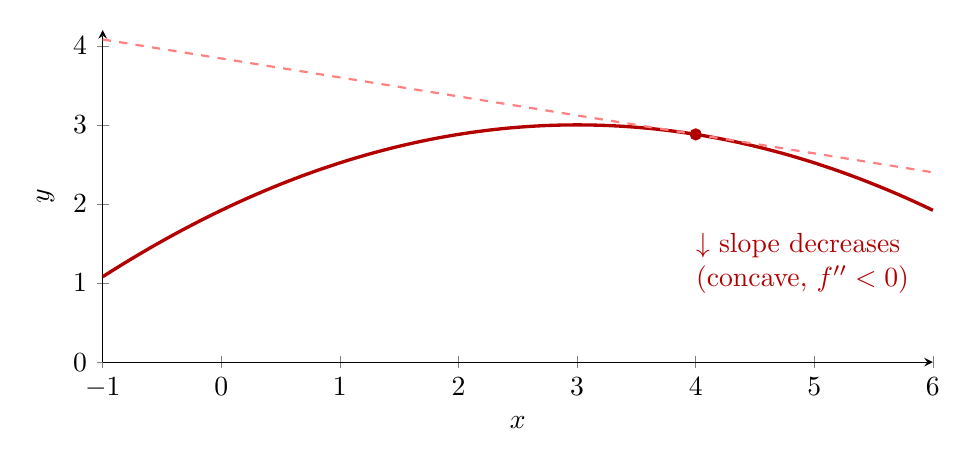
\begin{tikzpicture}
\begin{axis}[
  width=\linewidth, height=5.8cm,
  xmin=-1, xmax=6, ymin=0, ymax=4.2,
  axis lines=left, xlabel={$x$}, ylabel={$y$},
  domain=-1:6, samples=200, clip=false
]
\addplot[very thick, color=red!70!black] {3 - 0.12*(x-3)^2};
\addplot[thick, dashed, color=red!50!white] {3.84 - 0.24*x};
\addplot[only marks, mark=*, mark size=2pt, color=red!70!black] coordinates {(4,2.88)};
\node[align=left, text=red!70!black] at (axis cs:4.9,1.25) {$\downarrow$ slope decreases\\(concave, $f''<0$)};
\end{axis}
\end{tikzpicture}
\end{minipage}
\tcblower
If $f'(x_0)=0$ and $f''(x_0)<0$, $x_0$ is a \emph{local maximum}.  
Geometrically: the slope is decreasing; $f'$ switches from $+$ to $-$ across the peak (Ch.\ 9.2–9.4).
\end{tcolorbox}

\begin{tcolorbox}[sidebyside, righthand width=0.42\textwidth, title=\textbf{Curvature \& Tangents}]
\begin{minipage}{0.56\textwidth}
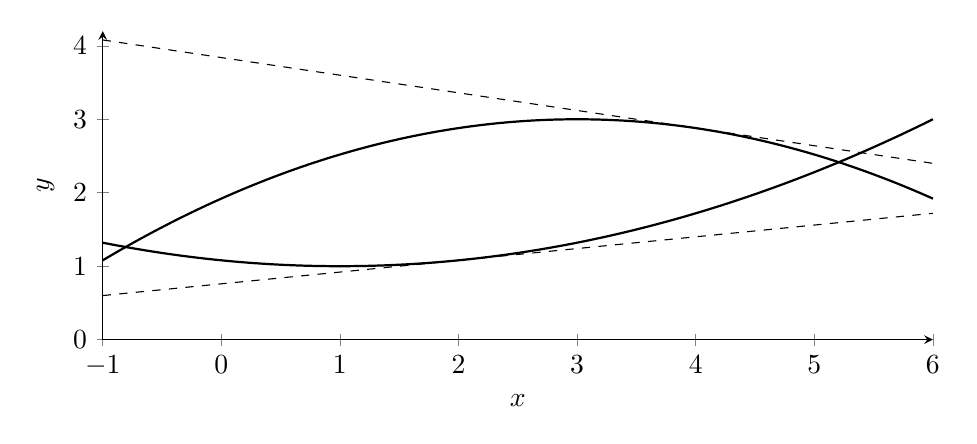
\begin{tikzpicture}
\begin{axis}[
  width=\linewidth, height=5.5cm,
  xmin=-1, xmax=6, ymin=0, ymax=4.2,
  axis lines=left, xlabel={$x$}, ylabel={$y$},
  legend style={at={(0.02,0.98)},anchor=north west, draw=none, fill=none},
  domain=-1:6, samples=200, clip=false
]
\addplot[thick] {1 + 0.08*(x-1)^2};
\addplot[dashed] {0.76 + 0.16*x};
\addplot[thick] {3 - 0.12*(x-3)^2};
\addplot[dashed] {3.84 - 0.24*x};
\end{axis}
\end{tikzpicture}
\end{minipage}
\tcblower
If $f'(x_0)=0$ and $f''(x_0)>0$ (convex), $x_0$ is a local minimum; if $f''(x_0)<0$ (concave), it’s a local maximum. Use the sign-change of $f'$ when $f''(x_0)=0$.
\end{tcolorbox}




%=============================================
% Figure 2: Risk-Averse Utility and Certainty Equivalent (COLOR)
%=============================================
\begin{figure}[ht]
\centering
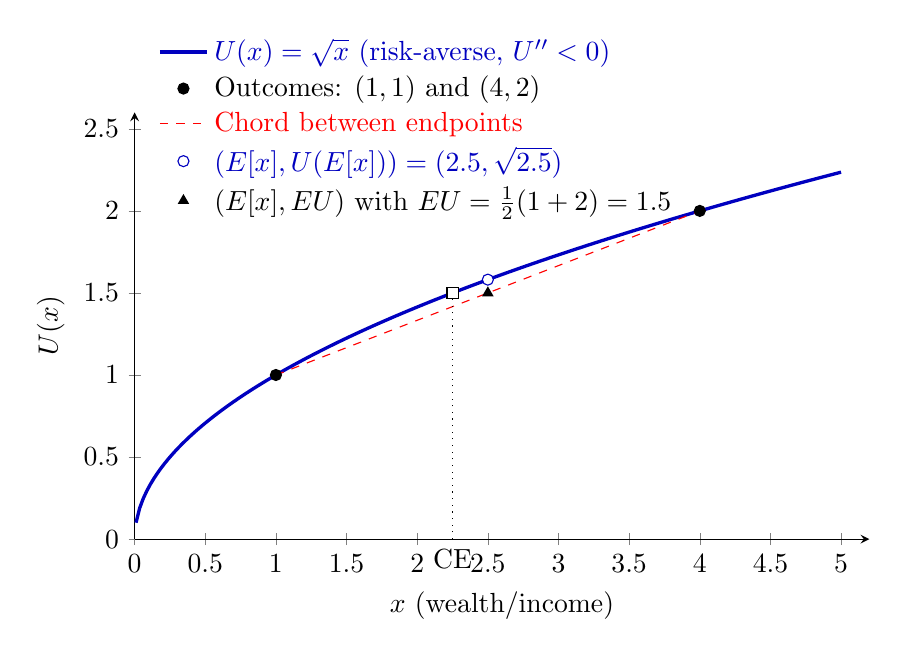
\begin{tikzpicture}
\begin{axis}[
  width=0.9\textwidth,
  height=7cm,
  xmin=0, xmax=5.2,
  ymin=0, ymax=2.6,
  axis lines=left,
  xlabel={$x$ (wealth/income)}, ylabel={$U(x)$},
  legend style={at={(0.02,1.2)},anchor=north west, draw=none, fill=none},
  legend cell align=left,
  domain=0.01:5, samples=200, clip=false
]
% Risk-averse utility (blue)
\addplot[very thick, color=blue!75!black] {sqrt(x)};
\addlegendentry{\textcolor{blue!75!black}{$U(x)=\sqrt{x}$ (risk-averse, $U''<0$)}}

% Endpoints of a 50-50 gamble (black dots)
\addplot[only marks, mark=*, color=black] coordinates {(1,1) (4,2)};
\addlegendentry{\textcolor{black}{Outcomes: $(1,1)$ and $(4,2)$}}

% Chord (gray dashed): y = (x+2)/3 on [1,4]
\addplot[dashed, color=red, domain=1:4] {(x+2)/3};
\addlegendentry{\textcolor{red}{Chord between endpoints}}

% (E[x], U(E[x])) shown as white-filled blue dot
\addplot[only marks, mark=*, mark options={fill=white}, color=blue!75!black]
  coordinates {(2.5,{sqrt(2.5)})};
\addlegendentry{\textcolor{blue!75!black}{$(E[x],U(E[x]))=(2.5,\sqrt{2.5})$}}

% (E[x], EU) shown as black triangle
\addplot[only marks, mark=triangle*, color=black]
  coordinates {(2.5,1.5)};
\addlegendentry{\textcolor{black}{$(E[x],EU)$ with $EU=\tfrac12(1+2)=1.5$}}

% Certainty equivalent: sqrt(CE)=1.5 -> CE=2.25 (dotted line + white-filled square)
\addplot[dotted, color=black] coordinates {(2.25,0) (2.25,1.5)};
\addplot[only marks, mark=square*, mark options={fill=white}, color=black]
  coordinates {(2.25,1.5)};
\node[text=black] at (axis cs:2.25,-0.12) {CE};

\end{axis}
\end{tikzpicture}
\caption{Risk Aversion: For a 50--50 gamble between $x=1$ and $x=4$, $EU=1.5 < U(E[x])=\sqrt{2.5}$. The certainty equivalent (CE $=2.25$) is less than $E[x]=2.5$.}
\end{figure}







\begin{tcolorbox}[sidebyside, righthand width=0.44\textwidth, title=\textbf{Risk Aversion \& CE}]
\begin{minipage}{0.54\textwidth}
\begin{tikzpicture}
\begin{axis}[
  width=\linewidth, height=6.2cm,
  xmin=0, xmax=5.2, ymin=0, ymax=2.6,
  axis lines=left, xlabel={$x$ (wealth)}, ylabel={$U(x)$},
  domain=0.01:5, samples=200, clip=false
]
% Utility curve
\addplot[very thick, color=blue!70!black] {sqrt(x)};

% Gamble endpoints
\addplot[only marks, mark=*, color=black] coordinates {(1,1) (4,2)};

% Chord between endpoints: y = (x+2)/3 on [1,4]
\addplot[dashed, color=gray, domain=1:4] {(x+2)/3};

% Expected wealth vs. utility points
\addplot[only marks, mark=*, mark options={fill=white}, color=blue!70!black]
  coordinates {(2.5,{sqrt(2.5)})}; % (E[x], U(E[x]))
\addplot[only marks, mark=triangle*, color=black]
  coordinates {(2.5,1.5)};          % (E[x], EU)

% Certainty equivalent: CE solves sqrt(CE)=1.5 => CE=2.25
\addplot[dotted, color=black] coordinates {(2.25,0) (2.25,1.5)};
\addplot[only marks, mark=square*, mark options={fill=white}, color=black]
  coordinates {(2.25,1.5)};
\node at (axis cs:2.25,-0.12) {CE};

\end{axis}
\end{tikzpicture}
\end{minipage}
\tcblower
Concavity ($U''<0$) $\Rightarrow$ diminishing marginal utility (Ch.\ 9.3).\\
Jensen: $U(E[x])\ge E[U(x)]$ so the certainty equivalent CE solving $U(\text{CE})=EU$ satisfies $\text{CE}<E[x]$.\\
The vertical gap to the chord is the \emph{risk premium}.
\end{tcolorbox}


%=========================================
% Figure 3: Risk-Loving Utility (for contrast) — COLOR
%=========================================
\begin{figure}[ht]
\centering
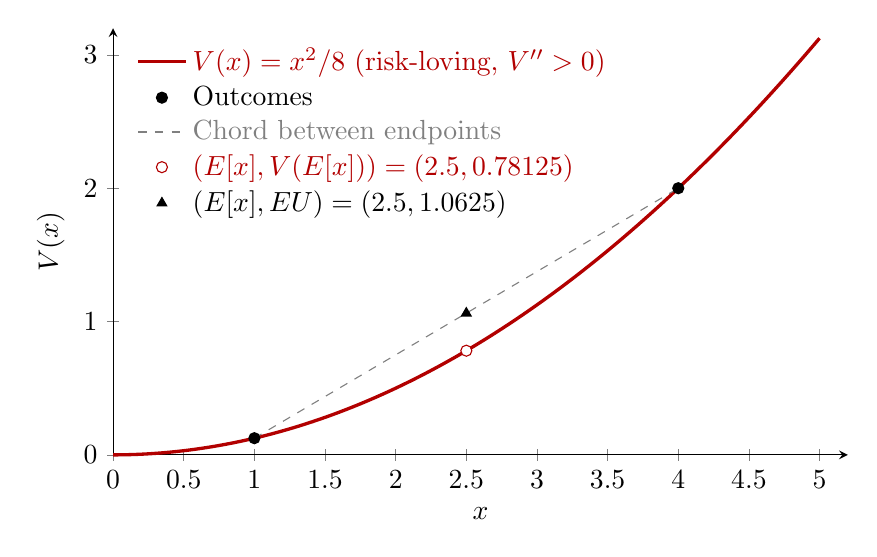
\begin{tikzpicture}
\begin{axis}[
  width=0.9\textwidth,
  height=7cm,
  xmin=0, xmax=5.2,
  ymin=0, ymax=3.2,
  axis lines=left,
  xlabel={$x$}, ylabel={$V(x)$},
  legend style={at={(0.02,0.98)},anchor=north west, draw=none, fill=none},
  legend cell align=left,
  domain=0:5, samples=200, clip=false
]
% Risk-loving (convex) utility, scaled (red)
\addplot[very thick, color=red!70!black] {(x^2)/8};
\addlegendentry{\textcolor{red!70!black}{$V(x)=x^2/8$ (risk-loving, $V''>0$)}}

% Outcomes 1 and 4 (black dots)
\addplot[only marks, mark=*, mark size=2pt, color=black] coordinates {(1,0.125) (4,2)};
\addlegendentry{\textcolor{black}{Outcomes}}

% Chord between endpoints: y = -0.5 + 0.625 x on [1,4] (gray dashed)
\addplot[dashed, color=gray, domain=1:4] {-0.5 + 0.625*x};
\addlegendentry{\textcolor{gray}{Chord between endpoints}}

% Expected wealth point (white-filled red dot): (E[x], V(E[x])) = (2.5, 0.78125)
\addplot[only marks, mark=*, mark size=2pt, mark options={fill=white}, color=red!70!black]
  coordinates {(2.5,0.78125)};
\addlegendentry{\textcolor{red!70!black}{$(E[x],V(E[x]))=(2.5,0.78125)$}}

% Expected utility EU = 0.5*(0.125+2) = 1.0625 at x=2.5 (black triangle)
\addplot[only marks, mark=triangle*, color=black]
  coordinates {(2.5,1.0625)};
\addlegendentry{\textcolor{black}{$(E[x],EU)=(2.5,1.0625)$}}

% (Optional) Show CE where V(CE) = EU: CE = sqrt(8.5) ≈ 2.9155
% \addplot[dotted, color=black] coordinates {(2.9155,0) (2.9155,1.0625)};
% \addplot[only marks, mark=square*, mark options={fill=white}, color=black]
%   coordinates {(2.9155,1.0625)};
% \node[text=black] at (axis cs:2.9155,-0.12) {CE};

\end{axis}
\end{tikzpicture}
\caption{Risk Loving: $EU>V(E[x])$, reflecting preference for risk when $V''>0$.}
\end{figure}



\begin{tcolorbox}[sidebyside, righthand width=0.44\textwidth, title=\textbf{Risk Loving (contrast)}]
\begin{minipage}{0.54\textwidth}
\begin{tikzpicture}
\begin{axis}[
  width=\linewidth, height=6.2cm,
  xmin=0, xmax=5.2, ymin=0, ymax=3.2,
  axis lines=left, xlabel={$x$}, ylabel={$V(x)$},
  domain=0:5, samples=200, clip=false
]
% Utility curve (convex)
\addplot[very thick, color=red!70!black] {(x^2)/8};

% Gamble endpoints
\addplot[only marks, mark=*, color=black] coordinates {(1,0.125) (4,2)};

% Chord between endpoints: y = -0.5 + 0.625 x on [1,4]
\addplot[dashed, color=gray, domain=1:4] {-0.5 + 0.625*x};

% Expected value vs utility points
\addplot[only marks, mark=*, mark options={fill=white}, color=red!70!black]
  coordinates {(2.5,0.78125)}; % (E[x], V(E[x])) with 2.5^2/8 = 0.78125
\addplot[only marks, mark=triangle*, color=black]
  coordinates {(2.5,1.0625)};  % (E[x], EU) with 0.5*(0.125+2) = 1.0625
% CE where V(CE) = EU = 1.0625 -> CE = sqrt(8.5) ≈ 2.91548
\addplot[dotted, color=black] coordinates {(2.9155,0) (2.9155,1.0625)};
\addplot[only marks, mark=square*, mark options={fill=white}, color=black]
  coordinates {(2.9155,1.0625)};
\node at (axis cs:2.9155,-0.12) {CE};

\end{axis}
\end{tikzpicture}
\end{minipage}
\tcblower
With convex $V$ ($V''>0$), the inequality reverses: $V(E[x])\le E[V(x)]$ (Ch.\ 9.3).\\
Risk lovers have $\text{CE}>E[x]$. Curvature alone flips preferences over lotteries vs.\ their mean.
\end{tcolorbox}




\section{Second-Derivative Test; Necessary vs. Sufficient Conditions; Profit Maximization}
\subsection*{Second-derivative test}
If $f$ is twice differentiable and $f'(x_0)=0$:
\[
\begin{cases}
f''(x_0)<0 \Rightarrow x_0 \text{ is a relative maximum},\\[2pt]
f''(x_0)>0 \Rightarrow x_0 \text{ is a relative minimum},\\[2pt]
f''(x_0)=0 \Rightarrow \text{inconclusive (use higher derivatives or the sign-change test).}
\end{cases}
\]

\subsection*{Necessary vs. sufficient}
\begin{itemize}[leftmargin=1.5em]
\item $f'(x_0)=0$ is a \emph{necessary} interior condition (first-order condition, FOC).
\item Together with $f''(x_0)\lessgtr 0$, we obtain a \emph{sufficient} condition (second-order condition, SOC) for a local max/min.
\end{itemize}

\subsection*{Application: profit maximization and the MR=MC rule}
Let total revenue $R(Q)$ and total cost $C(Q)$ be differentiable; profit $\pi(Q)=R(Q)-C(Q)$. The FOC
\[
\pd{\pi}{Q}=R'(Q)-C'(Q)=0 \quad\Longleftrightarrow\quad MR=MC
\]
pins down \emph{candidates}. The SOC for a maximum is $\pi''(Q)=R''(Q)-C''(Q)<0$ at the candidate. 

\begin{example}[Profit with a cubic cost]
Suppose $R(Q)=1200Q-2Q^2$ and $C(Q)=Q^3-61.25Q^2+1528.5Q+2000$. Then
\[
\pi'(Q)=R'(Q)-C'(Q)=(1200-4Q)-(3Q^2-122.5Q+1528.5)= -3Q^2+118.5Q-328.5.
\]
Setting $\pi'(Q)=0$ gives two stationary outputs (use quadratic formula). The SOC
\[
\pi''(Q)=R''(Q)-C''(Q)=-4-(6Q-122.5)=-6Q+118.5
\]
selects the one with $\pi''(Q)<0$ as the profit maximum. Always confirm the economic domain ($Q\ge0$) and compare profit values if boundaries matter.
\end{example}

\begin{remark}[Upward-sloping MR can occur]
When $AR(Q)$ is strictly convex on a segment, $MR(Q)=AR(Q)+Q\cdot AR'(Q)$ can slope upward on that segment because the $Q\,AR'(Q)$ term can dominate; nonetheless, MR=MC must still hold at an interior maximum, along with $\pi''<0$.
\end{remark}




%=========================================
% Figure 4: MR–MC Geometry with Linear Demand — COLOR
%=========================================
\begin{figure}[ht]
\centering
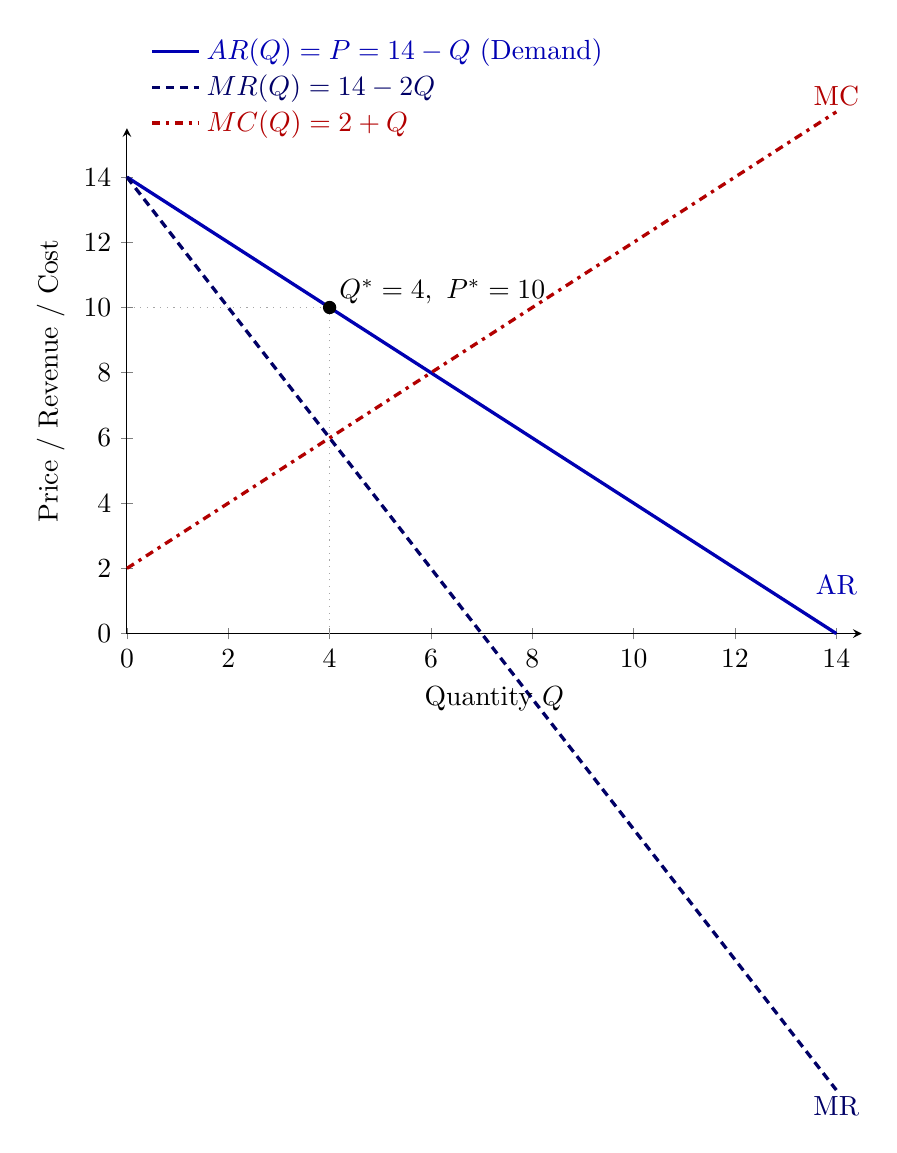
\begin{tikzpicture}
\begin{axis}[
  width=0.9\textwidth,
  height=8cm,
  xmin=0, xmax=14.5,
  ymin=0, ymax=15.5,
  axis lines=left,
  xlabel={Quantity $Q$}, ylabel={Price / Revenue / Cost},
  legend style={at={(0.02,1.2)},anchor=north west, draw=none, fill=none},
  legend cell align=left,
  domain=0:14, samples=200, clip=false
]

% AR (Demand): P = 14 - Q   (blue)
\addplot[very thick, color=blue!70!black] {14 - x};
\addlegendentry{\textcolor{blue!70!black}{$AR(Q)=P=14-Q$ (Demand)}}

% MR: 14 - 2Q                (blue dashed, lighter)
\addplot[very thick, densely dashed, color=blue!40!black] {14 - 2*x};
\addlegendentry{\textcolor{blue!40!black}{$MR(Q)=14-2Q$}}

% MC: 2 + Q                  (red dashdotted)
\addplot[very thick, dashdotted, color=red!70!black] {2 + x};
\addlegendentry{\textcolor{red!70!black}{$MC(Q)=2+Q$}}

% Profit-maximizing Q*: MR=MC -> 14-2Q = 2+Q => Q*=4; P*=10
\addplot[dotted, color=gray!70] coordinates {(4,0) (4,10)};
\addplot[dotted, color=gray!70] coordinates {(0,10) (4,10)};
\addplot[only marks, mark=*, mark size=2.2pt, color=black] coordinates {(4,10)};
\node[anchor=west, text=black] at (axis cs:4,10.5) {$Q^\ast=4,\ P^\ast=10$};

% Labels on curves (matching colors)
\node[text=blue!40!black] at (axis cs:14,-14.5) {MR};
\node[text=blue!70!black] at (axis cs:14,1.5) {AR};
\node[text=red!70!black]  at (axis cs:14,16.5)  {MC};

\end{axis}
\end{tikzpicture}
\caption{Monopoly choice: Interior optimum where $MR(Q^\ast)=MC(Q^\ast)$ with $P^\ast$ from the demand curve.}
\end{figure}




\begin{tcolorbox}[sidebyside, righthand width=0.42\textwidth, title=\textbf{MR–MC Geometry}]
\begin{minipage}{0.56\textwidth}
\begin{tikzpicture}
\begin{axis}[
  width=\linewidth, height=7.2cm,
  xmin=0, xmax=14.5, ymin=0, ymax=15.5,
  axis lines=left, xlabel={$Q$}, ylabel={Price / Rev / Cost},
  domain=0:14, samples=200, clip=false
]
\addplot[very thick, color=blue!70!black] {14 - x};          % AR (Demand)
\addplot[very thick, densely dashed, color=blue!40!black] {14 - 2*x}; % MR
\addplot[very thick, dashdotted, color=red!70!black] {2 + x}; % MC
\addplot[dotted, color=black] coordinates {(4,0) (4,10)};
\addplot[dotted, color=black] coordinates {(0,10) (4,10)};
\addplot[only marks, mark=*, color=black] coordinates {(4,10)};
\node[anchor=west] at (axis cs:4,10.2) {$Q^\ast=4,\ P^\ast=10$};
\end{axis}
\end{tikzpicture}
\end{minipage}
\tcblower
FOC (Ch.\ 9.4): $MR=MC$ selects candidates.  
SOC: $\pi''(Q)=R''(Q)-C''(Q)$. Here $R(Q)=14Q-Q^2\Rightarrow R''=-2$; with $MC=2+Q$ we get $C''=1$, so $\pi''=-3<0$—a strict local maximum.  
Always compare with boundaries (capacity, $Q\ge0$) for absolute optimality.
\end{tcolorbox}


\section{Maclaurin and Taylor Series (Approximations and Remainders)}
\subsection*{Motivation}
When $f''(x_0)=0$ (or higher derivatives vanish), the standard second-derivative test is inconclusive. Taylor expansions provide a principled way to examine higher-order curvature and to build local polynomial approximations.

\subsection*{Factorials and notation}
For $n\in\mathbb{N}$, $n!=n(n-1)\cdots 2\cdot1$ with $0!\equiv1$. We write $f^{(k)}$ for the $k$-th derivative.

\subsection*{Maclaurin expansion (around $0$)}
If $f$ is infinitely differentiable at $0$, its Maclaurin polynomial of order $n$ is
\[
P_n(x)= f(0)+\frac{f'(0)}{1!}x+\frac{f''(0)}{2!}x^2+\cdots+\frac{f^{(n)}(0)}{n!}x^n.
\]
\emph{Example.} If $f(x)=2+4x+3x^2$, then $f(0)=2$, $f'(0)=4$, $f''(0)=6$, so its Maclaurin series reproduces $f$ exactly.

\subsection*{Taylor expansion (around $x_0$)}
More generally,
\[
f(x)= f(x_0)+\frac{f'(x_0)}{1!}(x-x_0)+\frac{f''(x_0)}{2!}(x-x_0)^2+\cdots+\frac{f^{(n)}(x_0)}{n!}(x-x_0)^n+R_n(x),
\]
where the \emph{Lagrange remainder} is
\[
R_n(x)=\frac{f^{(n+1)}(p)}{(n+1)!}(x-x_0)^{n+1}\quad\text{for some }p\text{ between }x\text{ and }x_0.
\]

\begin{example}[Non-polynomial approximation]
Expand $\phi(x)=\dfrac{1}{1+x}$ around $x_0=1$ up to order $n=4$.
Compute derivatives $\phi^{(k)}(x)=(-1)^k k!(1+x)^{-(k+1)}$. Evaluate at $x_0=1$ and substitute into Taylor's formula to obtain a quartic approximation plus $R_4(x)$.
This gives an excellent local approximation near $x_0=1$ and quantifies the error via $R_4$.
\end{example}

\begin{remark}[Linearization you will use a lot]
For small $\Delta$, $f(x_0+\Delta)\approx f(x_0)+f'(x_0)\Delta$. This is the \emph{tangent-line} (first-order) approximation used constantly in comparative statics and elasticities.
\end{remark}

\section{The $n$th-Derivative Test for Relative Extremum of One Variable}
When lower-order derivative tests fail (e.g., $f'(x_0)=0$ and $f''(x_0)=0$), Taylor's theorem yields a powerful generalization.

\begin{proposition}[General $n$th-derivative test]
Let $f$ be $n$ times continuously differentiable near $x_0$ with
\[
f'(x_0)=f''(x_0)=\cdots=f^{(n-1)}(x_0)=0,\qquad f^{(n)}(x_0)\ne0.
\]
\begin{itemize}[leftmargin=1.5em]
\item If $n$ is \emph{even} and $f^{(n)}(x_0)>0$, then $x_0$ is a relative \emph{minimum}.
\item If $n$ is \emph{even} and $f^{(n)}(x_0)<0$, then $x_0$ is a relative \emph{maximum}.
\item If $n$ is \emph{odd}, then $x_0$ is an \emph{inflection point} (no extremum).
\end{itemize}
\end{proposition}

\begin{example}[Degenerate second derivative]
Consider $f(x)=x^4$. Then $f'(0)=0$, $f''(0)=0$, $f^{(3)}(0)=0$, $f^{(4)}(0)=24>0$. The first nonzero derivative is fourth and positive $\Rightarrow$ $x=0$ is a (flat) local minimum.
\end{example}

\section*{Boundary and corner solutions (one dimension)}
If the feasible set is a closed interval $[a,b]$, compare interior stationary values with $f(a)$ and $f(b)$. If the optimum occurs at $a$ or $b$, the FOC $f'=0$ need not hold: the Kuhn--Tucker logic in one dimension reduces to checking the boundary.

\section*{A checklist for single-variable optimization}
\begin{enumerate}[leftmargin=1.5em]
\item Specify objective $f(x)$ and feasible domain $\mathcal{D}$ (include units and economic meaning).
\item Compute $f'(x)$, solve $f'(x)=0$ for interior candidates; include any points where $f'$ is undefined but $x\in\mathcal{D}$.
\item Classify each candidate: use the second-derivative test; if inconclusive, use the first-derivative sign change or the $n$th-derivative test.
\item Evaluate $f$ at boundaries and compare with interior values for absolute optima.
\item In applications (profit, cost, utility), translate conditions back: MR=MC and $\pi''<0$ for a maximum; AC minimization at $Q$ where $AC'=0$ and $AC''>0$, etc.
\end{enumerate}

\newpage
\section*{Exercises}
\begin{enumerate}[leftmargin=1.5em]
\item Find and classify extrema of $f(x)=x^3-3x+1$. \emph{Answer:} $f'(x)=3x^2-3=0\Rightarrow x=\pm1$. $f''(x)=6x$: at $x=-1$, $f''<0$ (local max); at $x=1$, $f''>0$ (local min).
\item Let $AC(Q)=Q-4\ln Q +7$ for $Q>0$. Minimize $AC$. \emph{Answer:} $AC'(Q)=1-4/Q=0\Rightarrow Q^\ast=4$. $AC''(Q)=4/Q^2>0$, so $Q^\ast$ is a strict minimum.
\item (Risk) For $U(x)=\sqrt{x}$ and a fair $50$--$50$ bet between $10$ and $20$, compare $EU$ with $U(E[x])$. \emph{Answer:} $EU=\tfrac12(\sqrt{10}+\sqrt{20})<\sqrt{15}=U(15)$ (risk-averse).
\item (Degenerate curvature) Classify $f(x)=x^6-3x^4$. \emph{Answer:} $f'(x)=6x^5-12x^3=6x^3(x^2-2)$ gives $x\in\{0,\pm\sqrt{2}\}$. $f''(x)=30x^4-36x^2$: at $x=0$, $f''=0$ (use higher order: $f^{(4)}(0)=-72<0$ $\Rightarrow$ local maximum at $0$). At $\pm\sqrt{2}$, $f''>0$ $\Rightarrow$ local minima.
\end{enumerate}

\section*{References}
\begin{itemize}[leftmargin=1.5em]
\item Alpha C. Chiang and Kevin Wainwright (2005), \emph{Fundamental Methods of Mathematical Economics}, 4th ed.
\item Carl P. Simon and Lawrence Blume (1994), \emph{Mathematics for Economists}, Chs. on calculus and optimization.
\item Hal R. Varian, \emph{Intermediate Microeconomics}, sections on profit maximization and cost minimization.
\item Knut Syds{\ae}ter, Peter Hammond, et al., \emph{Essential Mathematics for Economic Analysis}, single-variable optimization chapters.
\end{itemize}

\end{document}
